%課題研究レジュメテンプレート ver. 1.0

\documentclass[uplatex]{jsarticle}
\usepackage[top=20mm,bottom=20mm,left=20mm,right=20mm]{geometry}
\usepackage[T1]{fontenc}
\usepackage{txfonts}
\usepackage{wrapfig}
\usepackage[expert,deluxe]{otf}
\usepackage[dvipdfmx,hiresbb]{graphicx}

\makeatletter
  \renewcommand{\section}{%
    \if@slide\clearpage\fi
    \@startsection{section}{1}{\z@}%
    {\Cvs \@plus.5\Cdp \@minus.2\Cdp}% 前アキ
    {.5\Cvs \@plus.3\Cdp}% 後アキ
    %{\normalfont\Large\headfont\raggedright}}
    {\normalfont\raggedright}}

  \renewcommand{\subsection}{\@startsection{subsection}{2}{\z@}%
    {\Cvs \@plus.5\Cdp \@minus.2\Cdp}% 前アキ
    {.5\Cvs \@plus.3\Cdp}% 後アキ
    %{\normalfont\large\headfont}}
    {\normalfont}}

  \renewcommand{\subsubsection}{\@startsection{subsubsection}{3}{\z@}%
    {\Cvs \@plus.5\Cdp \@minus.2\Cdp}%
    {\z@}%
    %{\normalfont\normalsize\headfont}}
    {\normalfont}}
\makeatother
%ここから上を編集する必要はない.





\title{\vspace{-14mm}twitterのアイコンによる拡散率を調べる}
\author{PMコース 矢吹研究室 1142016 井上 乃祐}
\date{}%日付を入れる必要はない.
\pagestyle{empty}%ページ番号は振らない.
\begin{document}
\maketitle





\section{研究の背景}

twitterは2006年に開始したサービスで,コミュニケーションツールのひとつとして利用され,月当たりのアクティブユーザは全世界で2億4100万人,投稿数は一日あたり約5億ツイートされていると言われ,多くの人に使われているソーシャル・ネットワーキング・サービスである\cite{inoue001}.その中にリツイートという機能があり,あるツイートの内容を自分のフォロワーの全員に拡散させる機能である.リツイートされるツイートには,ツイート内容という情報以外にアイコンや,ユーザーのIDなどの本質以外の情報も含まれる.
私は現在ツイッターを利用していて,フォローしているユーザーからリツイートが流れてくることがある.その流れてきたリツイートを見てみると,似たような内容でもリツイートされた回数に違いがあることに気づいた.そこで私は自分のプロフィールのアイコンが拡散率に影響があるのではないかと考えた.






\section{研究の目的}


twitterのアイコンが拡散率に影響があるかを調べ,情報の本質でないアイコン部分が本質に与える影響を調べる.








\section{プロジェクトマネジメントとの関連}

アイコンでの拡散率の違いが生じるのならば,企業のツイートを受け取る際にステークホルダにより早く情報を伝えることが出来ると言える.これは9つの知識エリアの中のリスク管理マネジメントと関連すると言えるだろう.





\section{リツイートされたデータを集める方法}



twitterのAPIを用いて,タイムラインに流れてきたリツイートのアイコンと,リツイート数,お気に入り数,フォロワー数,を自動で保存しデータを300個集める.

その後リツイートされたアイコンを,若い男性,中年の男性,年配の男性,子供の男の子,男複数,若い女性,中年の女性,年配の女性,子供の女の子,女複数,男女複数,初期アイコン,男アニメ,男アニメ複数,女アニメ,女アニメ複数,アニメ・マスコット,マスコット・キャラクター,無機物,自作の絵,動物・ペット,ロゴ・マーク,景色・風景,文字,食べ物の25要素でタグ付けする.

説明変数を25個のタグ付けしたデータ,目的変数をリツイート数/フォロワー数で重回帰分析をする.













\section{現在の進捗状況}

twitterのAPIを使ってリツイートされたデータを300個集め,それを表1のようにエクセルに入力した.さらにそのデータを説明変数を25個のタグ付けしたデータ,目的変数をリツイート数/フォロワー数で重回帰分析をした.

%\begin{wraptable}[行数]{r}{幅}%行数はオプションだが,調整しないとうまくいかない.
\begin{wraptable}[7]{r}{4cm}
\vspace*{-\intextsep}
\caption{}\label{サンプル表}
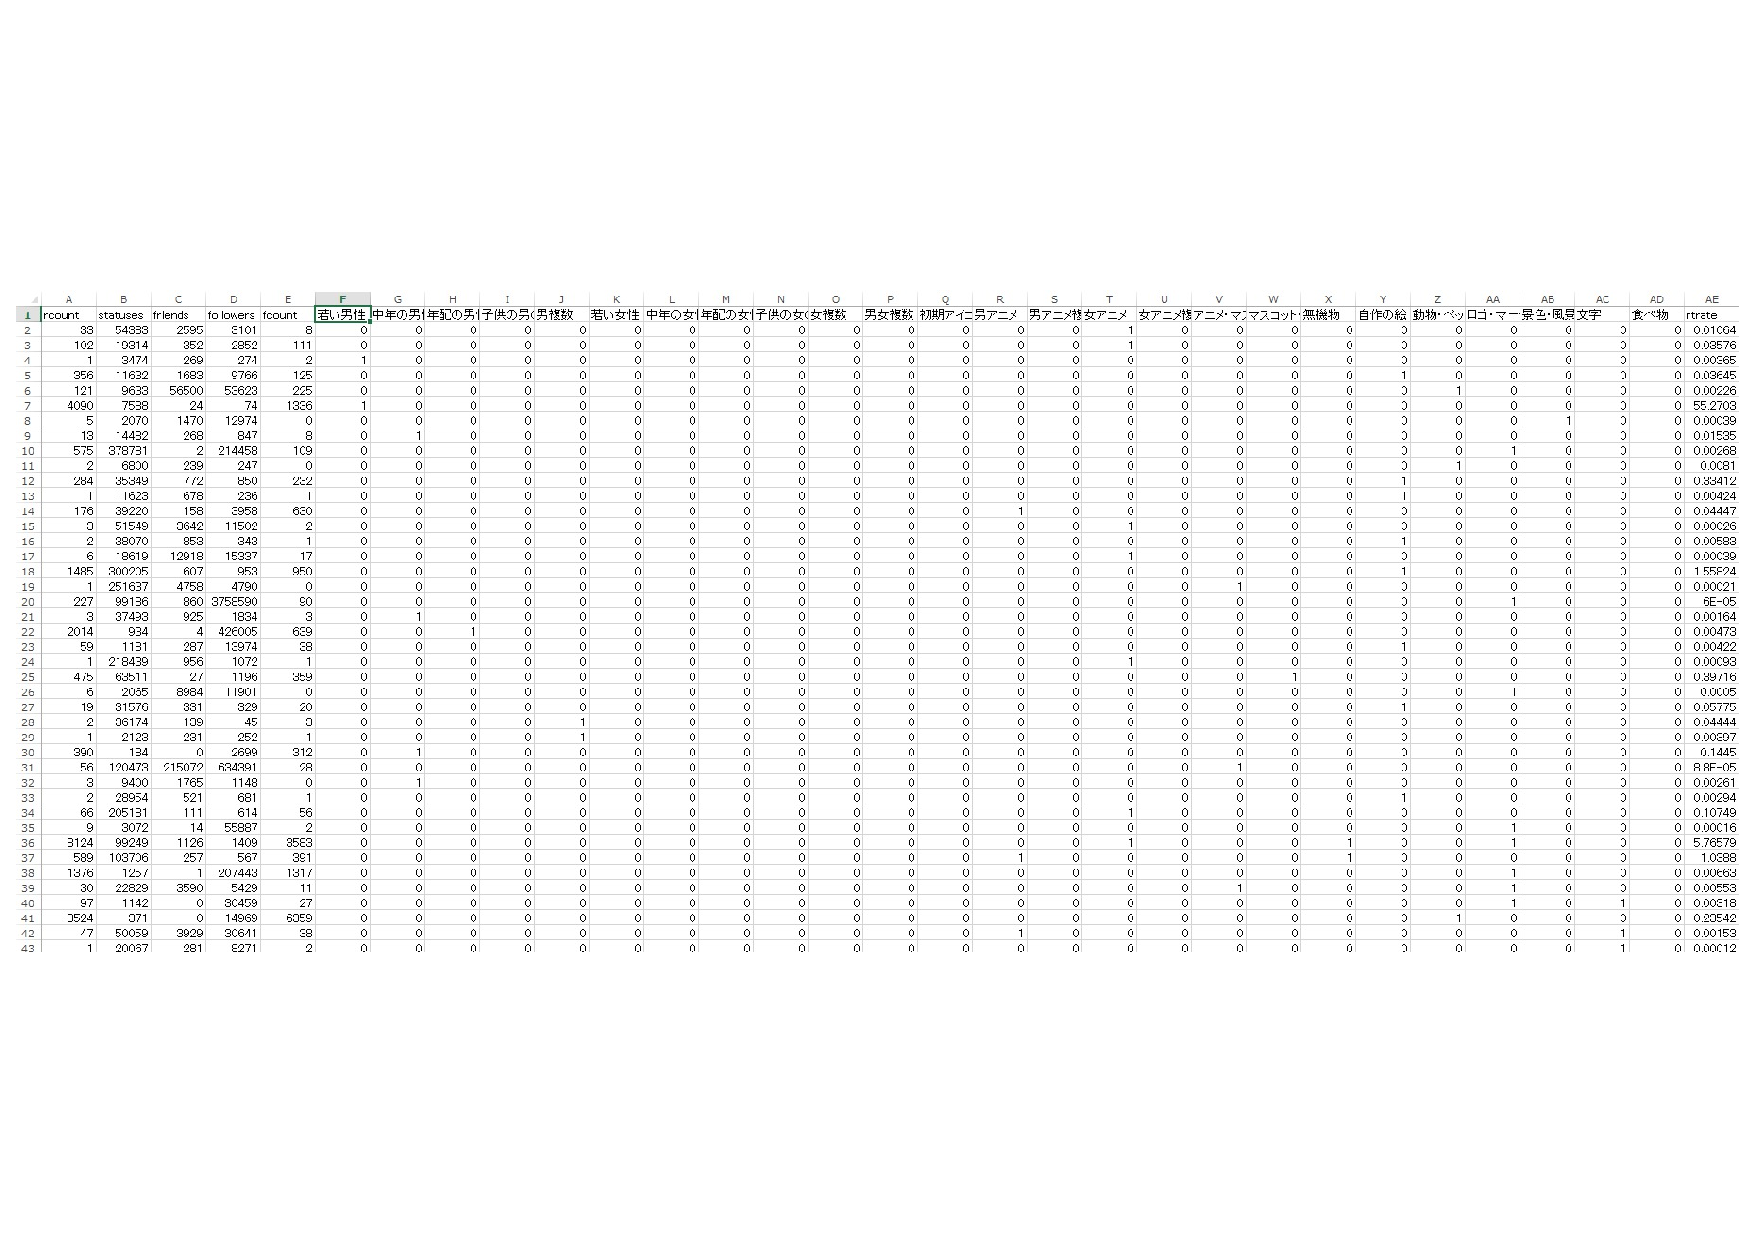
\includegraphics[width=5cm,clip]{rtdata.pdf}
\end{wraptable}


その中で拡散率を上げる可能性のあるものをいくつか見つけた.
その結果が図1である.

%\begin{wrapfigure}[行数]{r}{幅}%行数はオプションだが,調整しないとうまくいかない.
\begin{wrapfigure}[11]{r}{4cm}
\vspace*{-\intextsep}
%\includegraphics[width=図の幅,clip]{ファイル名}\label{参照用ラベル}
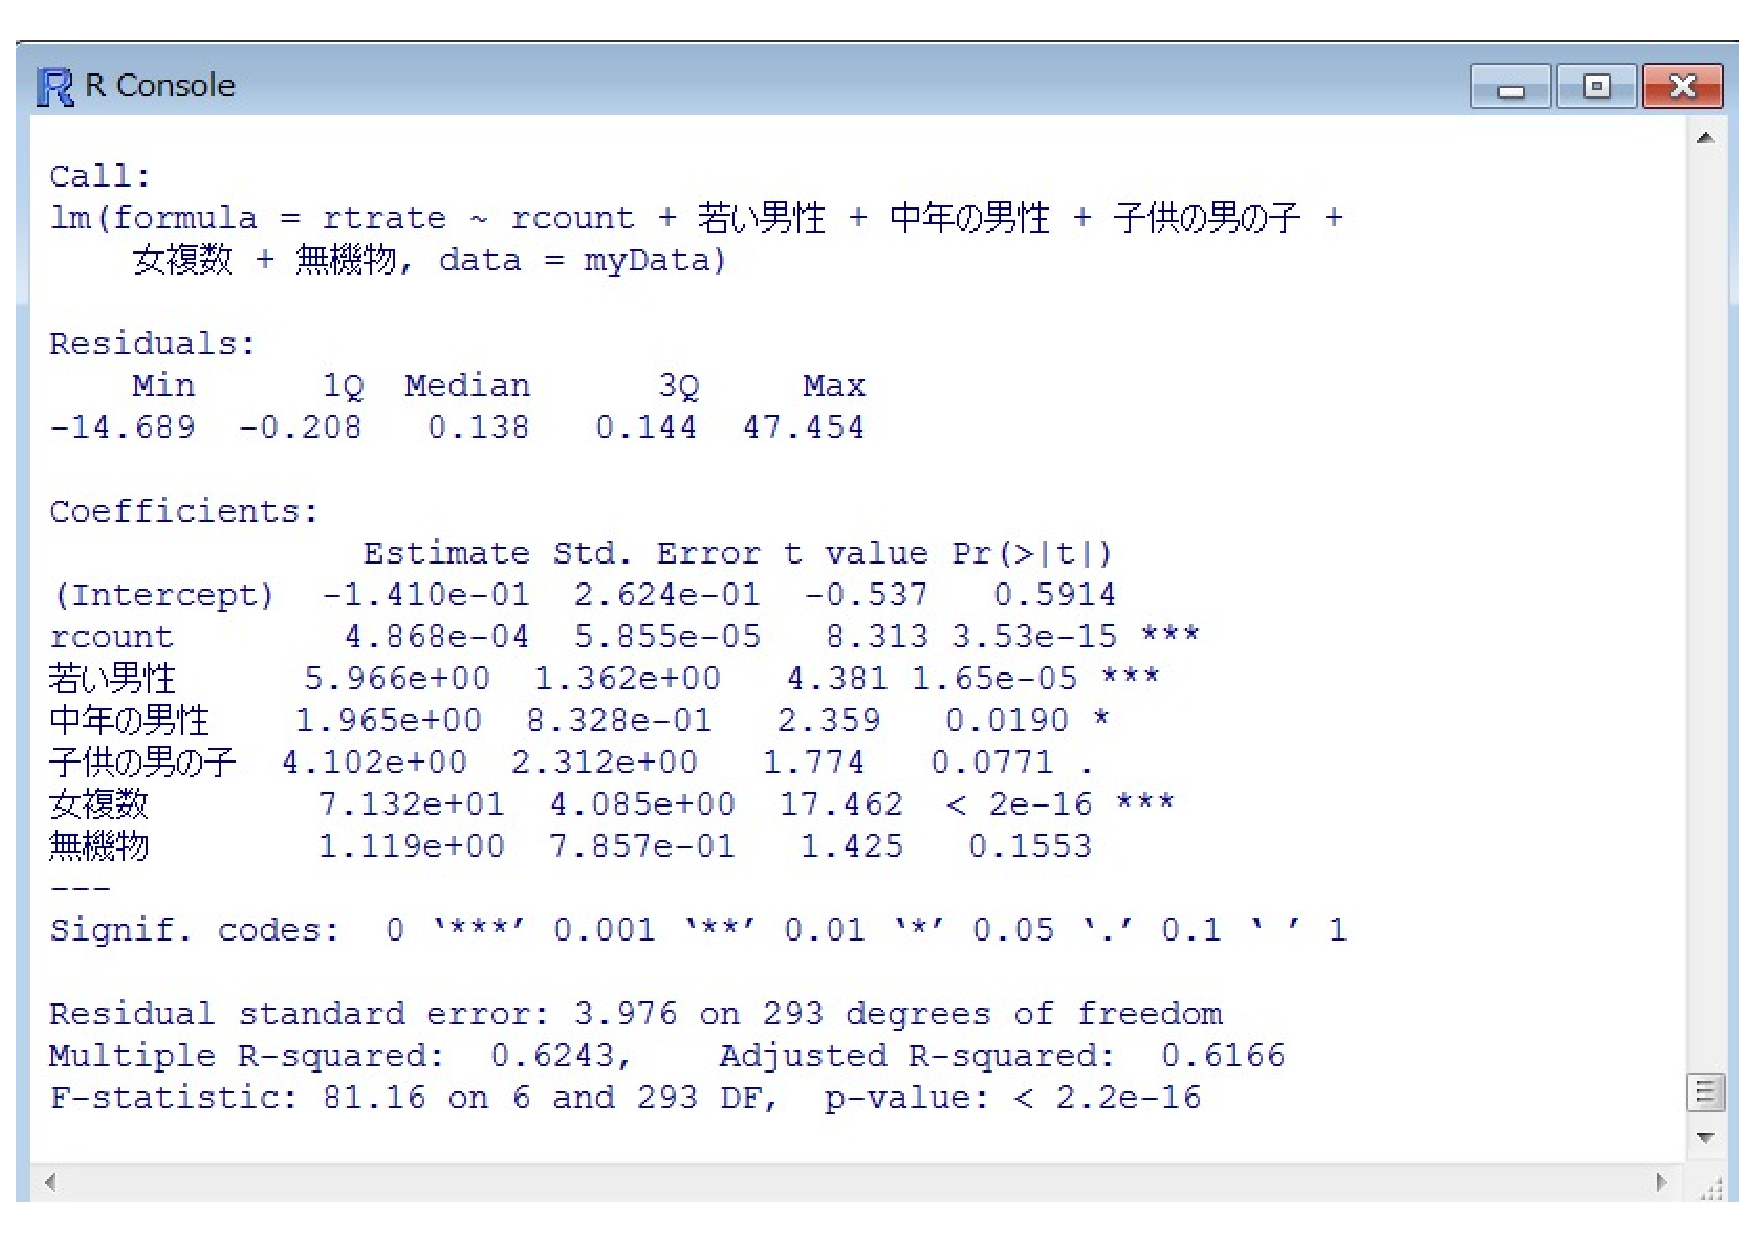
\includegraphics[width=5cm,clip]{images.pdf}
\caption{}\label{サンプル図}
\end{wrapfigure}


拡散率を上げる要素として一番影響があるのが若い男性,次に中年の男性,その次は子供の男の子であった.しかし,子供の男の子はデータ量が少ないため,その次の女性(複数)が影響があると結論付けた.

私は女性のほうが拡散率が高くなると予想していたが,結果は男性のアイコンの方が拡散率が高くなった.



\section{今後の計画}

以下のように研究を進める計画である.

\begin{enumerate}
\item タグ付けの項目をさらに増やして,細かい結果を調べる.
\item リツイートの画像を判別する際に画像処理のAPIを入れたが,画像の判別ミスが多く目立ったため,画像処理について平行して研究する.

\end{enumerate}

\bibliographystyle{junsrt}
\bibliography{biblio}%「biblio.bib」というファイルが必要.

\end{document}
